\documentclass[12pt]{article}
\usepackage[a4paper,margin=2.5cm]{geometry}
\usepackage{tikz}
\usepackage{xcolor}

\begin{document}

\section*{Alas dan Dua Busur Jangka}

% Alas AB = 6 cm. Titik C = (3.75, 3.31): berjarak 5 cm dari A
% dan 4 cm dari B, yaitu perpotongan kedua busur.
\begin{tikzpicture}[scale=1.1]
  \coordinate (A) at (0,0);
  \coordinate (B) at (6,0);
  \draw[thick] (A) -- (B);
  \node[below left] at (A) {$A$};
  \node[below right] at (B) {$B$};
  \begin{scope}
    \clip (-0.5,0) rectangle (6.5,4.5);
    \draw[dashed, blue] (A) circle (5);
    \draw[dashed, red] (B) circle (4);
  \end{scope}
  \fill (3.75,3.31) circle (2pt);
  \node[above] at (3.75,3.31) {$C$};
  \node[blue] at (1.2,3.8) {jari-jari 5 cm dari $A$};
  \node[red] at (5.3,3.8) {jari-jari 4 cm dari $B$};
\end{tikzpicture}

\section*{Segitiga Jadi: $AB = 6$ cm, $AC = 5$ cm, $BC = 4$ cm}

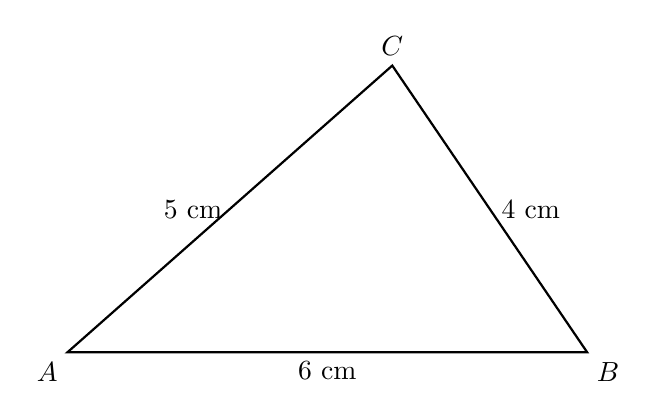
\begin{tikzpicture}[scale=1.1]
  \coordinate (A) at (0,0);
  \coordinate (B) at (6,0);
  \coordinate (C) at (3.75,3.31);
  \draw[thick] (A) -- (B) -- (C) -- cycle;
  \node[below left] at (A) {$A$};
  \node[below right] at (B) {$B$};
  \node[above] at (C) {$C$};
  \node[below] at (3,0) {$6$ cm};
  \node[left] at (1.9,1.65) {$5$ cm};
  \node[right] at (4.9,1.65) {$4$ cm};
\end{tikzpicture}

\end{document}
